\documentclass[12pt, oneside]{article}   	% use "amsart" instead of "article" for AMSLaTeX format
\usepackage{geometry}                		% See geometry.pdf to learn the layout options. There are lots.
\geometry{letterpaper}                   		% ... or a4paper or a5paper or ... 
%\geometry{landscape}                		% Activate for rotated page geometry
%\usepackage[parfill]{parskip}    		% Activate to begin paragraphs with an empty line rather than an indent
\usepackage{graphicx}				% Use pdf, png, jpg, or eps§ with pdflatex; use eps in DVI mode
\graphicspath{ {../figures/} }
								% TeX will automatically convert eps --> pdf in pdflatex		
\usepackage{amssymb}
\usepackage{amsmath}
\usepackage{hyperref}
\usepackage{float}
\usepackage[utf8]{inputenc}
\usepackage[english]{babel}
\usepackage[toc,page]{appendix}
% \usepackage[cache=false]{minted}

\usepackage{setspace}
\doublespace

% Move page number down
% \setlength{\footskip}{0.001cm}
% \pagenumbering{gobble}

%SetFonts

%SetFonts


\title{%
	Predicting Movie Ratings with Movie Posters}
\author{Christopher Pyles}
\date{May 13, 2020}							% Activate to display a given date or no date

\begin{document}

\maketitle

\section*{Abstract}

The efficacy of using movie posters as predictors of movie ratings is concerned with training both fully-connected and convolutional neural networks on poster images from The Movie Database, a community-managed movie database owned by TiVo. The ability to use such features as elements in a prediction model would aid in honing many prediction algorithms used by streaming services to recommend movies to their viewers. Neural networks are here used because they require the least data preprocessing and because they naturally extend to working with image data. To understand the value of these models compared to others, control models trained on other data about the movies, e.g. the synopsis and genre, are built and trained. These models include support vector, ridge, k-nearest neighbors, and decision tree classifiers. Various feature engineering and selection techniques are employed on these control models, including A/B testing to create features from the synopses. Principal components analysis is performed on the finalized dataset to consider the possibility of dimensionality reduction. The results of this analysis show that the poster predictors perform comparably worse than the control models, indicating that under these circumstances posters are likely not good predictors of ratings, and that further analysis with deep learning models or other classifiers should be performed to confirm this conclusion.

\newpage

\tableofcontents

\newpage

\section{Introduction}

The ability to predict the rating of a movie before its release would be a great asset to production companies. Ratings are generally correlated with the revenue made by a movie, as people tend to base their decisions of whether or not to see a movie on the reviews they read and the general attitude toward the movie. This analysis considers the use of movie posters as predictors of ratings, comparing the efficacy of this to classifiers built on other data about the movie.

Various techniques have been applied to the question of predicting movie ratings based on different types of data. Oghina et. al. \cite{oghina_predicting_2012} applied prediction algorithms to data from the Internet Movie Database (IMDb) and attempted to predict ratings based on social media. Their analysis is based on textual data from sources like YouTube and Twitter, which they used to extract other textual features that were used in the final predictive model. Navarathna et. al. \cite{navarathna_predicting_2014} consider a different model of movie rating prediction based on observations of moviegoers' faces and body language during a viewing experience. Other implementations of this problem include the problem of automatically predicting specific users' ratings, as discussed in Marović et. al. \cite{marovic_automatic_2011}, who use machine learning methods to predict these ratings in service of a recommendation algorithm.

The paper by Kudagamage et. al. \cite{kudagamage_data_2018} discussed an approach to the prediction of movies' success based in data mining techniques. This analysis looks at various geometric properties of its data, including spatial clustering, and how this relates to the success of a movie. Instead of predicting movies directly, movies are partitioned into four clusters representing most successful, successful, unsuccessful, and least successful movies. 

A natural extension of this research is demonstrated in Diao et. al. \cite{diao_jointly_2014}, which describes how ratings and review sentiments can be used to model movie recommendations. This model is again trained on IMDb data and thinks about how data scraped from the site on ratings and reviews can be used to build a recommendation algorithm. The ability to predict the ratings for a movie is a precursor to analyzing the market for the movie using such recommendation models, for example to predict how many streaming service users might watch this movie based on its predicted rating. 

In this analysis, the use of posters as predictors of ratings is examined, using both fully-connected and convolutional neural networks as models trained on the posters. Neural networks, as opposed to other types of classifiers, are used in this analyzes because they require the least data preprocessing and because they naturally extend to working with images, and the efficacy of convolutional neural networks as image predictors for a variety of problems has been shown again and again. As a control, models trained on other data about the movies, e.g. the synopsis and genre, are also trained and tested as a point of comparison against the poster-based models. Different types of classifiers are used for the control, and the best of them is used as the point of comparison. Exploratory data analysis and A/B testing are also used in service of building a set of features for these control models.

This project uses the programming language Python to perform the analysis and the neural networks are provided by the package keras with tensorflow as its backend. Packages including numpy, scikit-learn, matplotlib, seaborn, pandas, and datetime are used to manipulate the data, create plots, and interact with the keras models.

\section{Data}

The data used in this project is from \href{https://api.tmdb.org}{The Movie Database's (TMDb) API}. TMDb is a community-managed online database of movie and television data that is owned and operated by TiVo. The data queried covers movies released in 2018 in English, spanning many genres: Action, Adventure, Animation, Comedy, Crime, Documentary, Drama, Family, Fantasy, Histor, Horror, Music, Mystery, Romance, Science Fiction, TV Movie, Thriller, War, and Western. Figure \ref{fig:genre_barplot} shows the number of movies in each genre.

The data, after being queried, were joined into a single table and written to a CSV file. The columns of interest are described in Table \ref{table:cols_of_interest}. After dropping rows with missing values in the columns of interest, the data contained $n=2700$ rows.

\begin{table}
\begin{center}\begin{tabular}{c|l}
\textbf{Column} & \textbf{Description} \\ \hline
\texttt{id} & \textbf{primary key}, a unique ID number for each movie \\
\texttt{adult} & whether or not the movie is R+ rated \\
\texttt{genre\_ids} & list of genre ID numbers corresponding to \texttt{genres} table \\
\texttt{original\_language} & the language that the movie was originally released in \\
\texttt{original\_title} & the title of the movie \\
\texttt{overview} & movie synopsis \\
\texttt{release\_date} & the date of first release \\
\texttt{vote\_average} & average of rating votes on a 10-point scale \\
\texttt{vote\_count} & the number of votes \\
\texttt{poster\_path} & URL path to movie poster \\
\end{tabular}\end{center}
\caption{\label{table:cols_of_interest}Column descriptions for TMDb API data (the \texttt{movies} table).}
\end{table}

\subsection{Data Cleaning}

Cleaning the data for this project, after dropping missing values, involved rounding the \texttt{vote\_average} column, cleaning the synopsis strings, joining the \texttt{genres} and \texttt{movies} tables, and converting the movie posters into 140 $\times$ 92 $\times$ 3 arrays of RGB values.

The \texttt{vote\_average} column ($\mu = 6.628$, $\sigma = 1.939$) describes the variable of interest, representing the average rating across votes for a single movie. In this analysis, this column will be transformed from a continuous variable into an ordinal variable with possible values 1 to 10 by rounding the vote average to a whole number. After rounding, the distribution of ratings is provided in Figure \ref{fig:rating_barplot}.

\begin{figure}%[H]
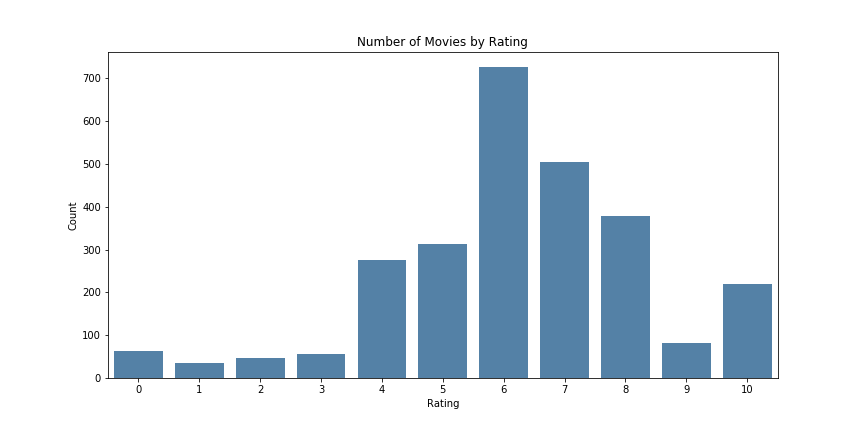
\includegraphics[width=\textwidth]{rating_barplot}
\caption{\label{fig:rating_barplot}Number of movies for each value of ratings, rounded from \texttt{vote\_average}.}
\end{figure}

To clean the movie synopses, all letters were transformed to lowercase, and any characters not matching the regex \texttt{[A-Za-z0-9 ]} were replaced with spaces.

The \texttt{genre\_ids} column is a list of genre IDs encoded as a string, so to start any empty lists, \texttt{"[]"}, were replaced with \texttt{NaN}. Then, the string were split into Python lists of IDs, and were joined with the \texttt{genres} table, so that \texttt{movies} had a column \texttt{genres} where each value is a list of genres for that movie. Figure \ref{fig:genre_barplot} shows the breakdown of movies by genre.

\begin{figure}%[H]
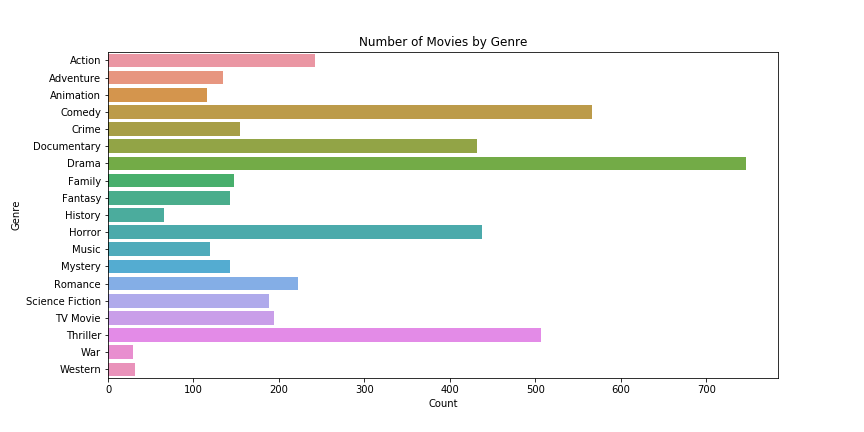
\includegraphics[width=\textwidth]{genre_barplot}
\caption{\label{fig:genre_barplot}Number of movies in each genre.}
\end{figure}

Lastly, each movie poster was downloaded from TMDb and stored as a 92 $\times$ 140 $\times$ 3 array in NumPy, stored as a .mat file. The structure of this file is analagous to a dictionary, where each key is a movie ID (as a string) and each value is the 3-D array of RGB values describing the poster.

\subsection{Exploratory Data Analysis}

Before modeling, a cursory analysis of the data yielded the interesting relationships:

\begin{itemize}

\item Figure \ref{fig:vote_count_by_rating} shows that vote count tends to increase logarithmically with rating until 8, after which it drops significantly. This demonstrates that having more votes tends to "bring down the curve."

\begin{figure}%[H]
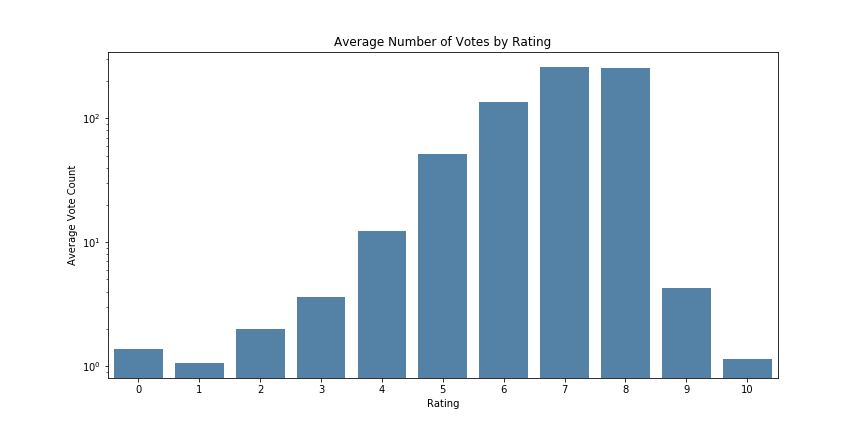
\includegraphics[width=\textwidth]{vote_count_by_rating}
\caption{\label{fig:vote_count_by_rating}Average vote count by rating.}
\end{figure}

\item There are significantly more non-adult movies than adult movies, as demonstrated in Figure \ref{fig:ratings_by_adult}. It is interesting to note that adult movies have a double-peak distribution with far less spread than do the non-adult movies.

\begin{figure}%[H]
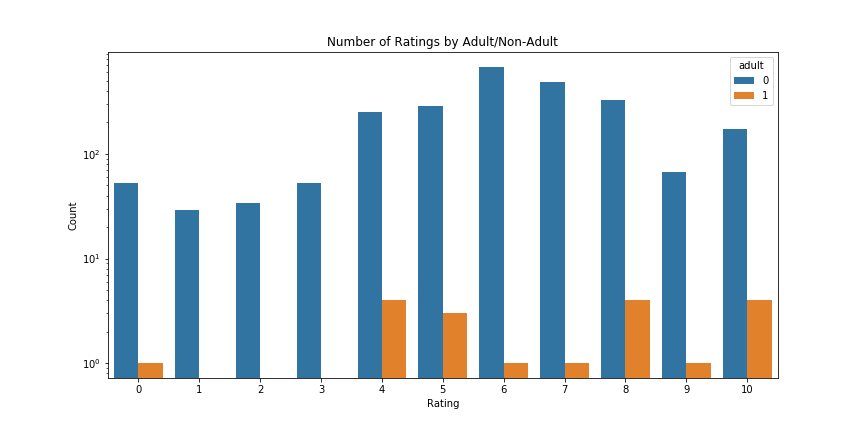
\includegraphics[width=\textwidth]{ratings_by_adult}
\caption{\label{fig:ratings_by_adult}Number of ratings by adult/non-adult.}
\end{figure}

\item Figure \ref{fig:ratings_by_genre} shows the distribution of ratings for each genre.

\begin{figure}%[H]
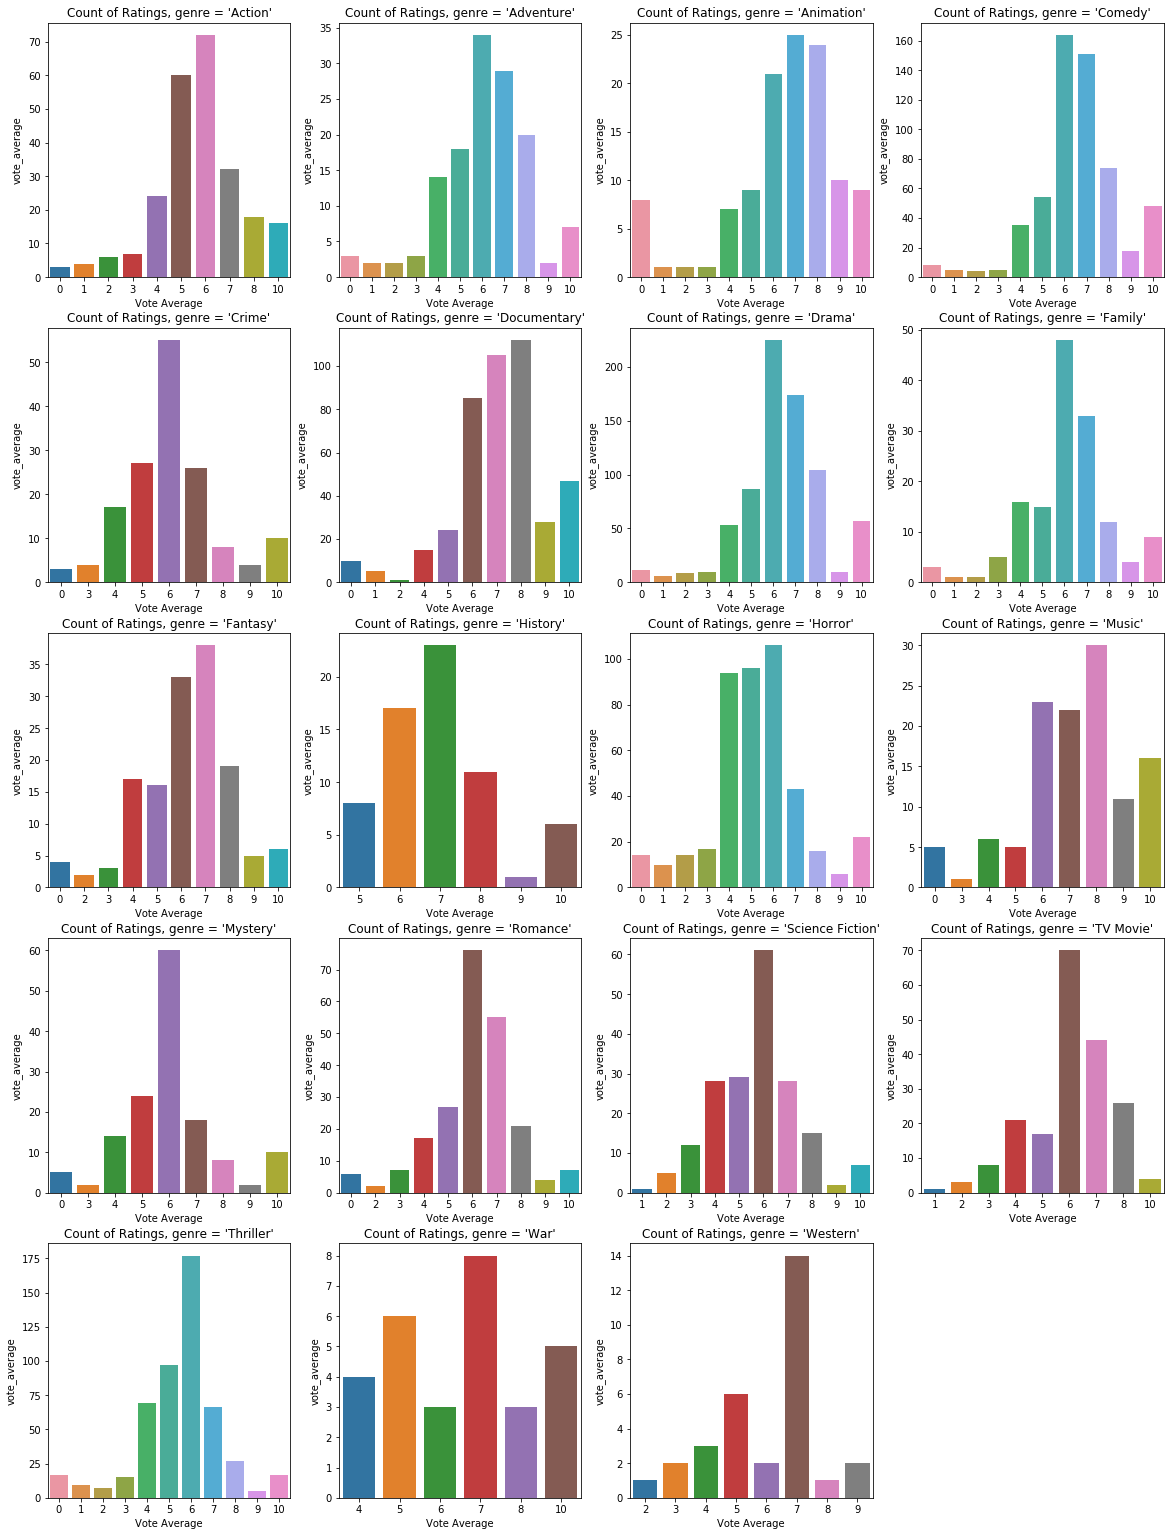
\includegraphics[height=0.9\textheight]{ratings_by_genre}
\caption{\label{fig:ratings_by_genre}Distribution of ratings by genre.}
\end{figure}

\item No discernible relationship is seen between the length of the overview and the movie's rating.

\item The distributions of ratings by release date day of week appear to be different in skew (Figure \ref{fig:ratings_dow}), indicating that this may be an important feature. No discernible relationship is seen between rating and day of month or month of release.

\begin{figure}%[H]
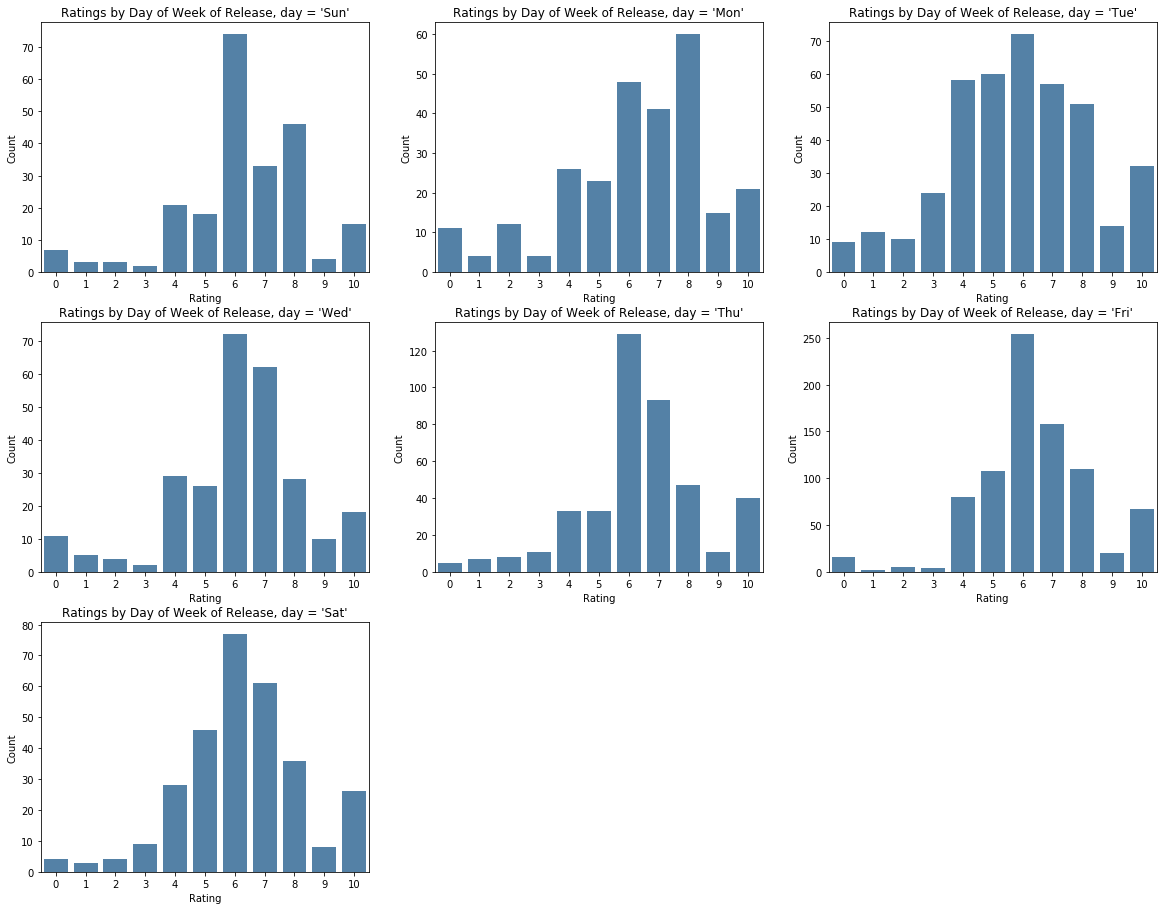
\includegraphics[width=\textwidth]{ratings_dow}
\caption{\label{fig:ratings_dow}Distribution of ratings by day of week of release.}
\end{figure}

\end{itemize}

\section{Analysis}

\subsection{Words in Synopses}
\label{section:words_in_synopses}

As the first part of this analysis, the statistical significance of the presence of different words in synopses is studied using hypothesis testing. The null hypothesis for this test is that the presence of a word does not affect the average rating, and the alternative is that the presence of the word results in an increase in rating. The test statistic used here is the aboslute difference between the mean rating of movies where the word is present in the synopsis and the movies where it is not. Under the null hypothesis, the truth value of a word being present in a synopsis is shuffled for each observation, so that same number of ``present''s is obtained. Then, the test statistic is computed and the p-value is calculated as the proportion of the test statistic values that are greater than or equal to the observed value for that word. Finally, those words whose p-values indicate statistical significance are added to the movies data as one-hot features, with a 1 in their column if the word is present in the synposis and a 0 otherwise. These dummy variables will be used as some of the features in the control model.

\subsection{Principal Components Analysis}
\label{section:pca}

After analyzing the presence of words in synopses, the dimensionality of the data is considered for reduction using principal components analysis (PCA). In this portion of the analysis, all of the features now in \texttt{movies} are analyzed via PCA in order to determine what proportion of the variance in the data can be explained using only a few principal components as a basis. This is accomplished with scikit-learn's \texttt{sklearn.decomposition.PCA} class. The principal components are considered only for the purpose of analyzing the variance of the data, and will not be used in modeling.

\subsection{Classification without Posters}
\label{section:class_no_posters}

The next step in the analysis is to attempt classification using the features in \texttt{movies} alone (i.e. without the posters). These include the columns described in Table \ref{table:cols_of_interest} and the words found in \S \ref{section:words_in_synopses} In this section, several different classification methods are tested, including a ridge classifier, a decision tree classifier, a support vector classifier (SVC), and a $k$-nearest neighbors (kNN) classifier. Each of these models is trained on training data from \texttt{movies} and evaluated using different error metrics on testing data from \texttt{movies}. Three different error metrics are used to evaluate each classifier: classification accuracy, root-mean-squared prediction error (RMSE), and mean absolute error (MAE). The last two, normally regression metrics, are used because the ratings are derived from continuous variables, and a classifier that classifies a movie closer to its rating than another is more accurate, and hit-miss accuracy does not account for this.

In order to select features, multiple methods are used and compared. The $k$ best features based on chi-squared statistics, ANOVA F-value, and mutual information are each selected and compared using tuned hyperparameters for each model. $k$ is also tuned using hyperparameter selection.

5-fold cross-validation (CV) is used to tune hyperparameters. The hyperparameters being tuned for each model are:
\begin{itemize}
\item ridge classifier: $\alpha$, the regularization strength
\item SVC: $C$, the regularization parameter (analagous to $\alpha^{-1}$ from the ridge classifier)
\item kNN classifier: the number of neighbors
\end{itemize}
These are the only hyperparameters tuned in this anlaysis because they most closely affect the accuracy of the models, mainly having to do with preventing overfitting. Hyperparameters are tuned individually for sets of features chosen by the different methods of feature selection described above. The model with the best CV error is chosen and trained on the training set using the corresponding features and evaluated using testing error.

\subsection{Classifying Movie Posters}
\label{section:class_posters}

In this portion, movie posters, stored as 3-tensors, are used as inputs to conlutional neural networks (CNNs) in order to classify the movie by rating. This section does not involve any features in \texttt{movies}. CNNs are trained on the 4-D array of all images and the classes encoded as dummy variables. The networks are compiled using categorical cross-entropy loss and the Adam optimization algorithm. They are evaluated as in \S \ref{section:class_no_posters}, using classification accuracy, RMSE, and MAE with 5-fold CV to determine the best network structure. The model with the best metrics is trained on the entire training set and evaluated on the test set.

\section{Results}

\subsection{Words in Synopses}
\label{section:words_results}

This analysis found that there were 110 words that were statistically significant in terms of the distribution of ratings, summarized in Table \ref{table:word_p_values} (cf. Appendix \ref{appendix:word_signif_table}) with their p-values. Each of these words was added as a feature to \texttt{movies} as dummy variables with 0-1 values indicating the presence of that word in the synopsis, resulting in the data points in \texttt{movies} becoming 141-dimensional. These new features will be used in prediction for the control models.

\subsection{Principal Components Analysis}
\label{section:pca_results}

PCA was performed on \textit{all} columns of \texttt{movies}, including both the word-significance dummy variables and some of the original columns listed in Table \ref{table:cols_of_interest}. PCA shows that only a few principal components (two, in fact) are required to account for almost 100\% of the variance in the data set, as demonstrated in Figures \ref{fig:scree_whole} and \ref{fig:scree_first_10} (the former shows all 141 principal components and the latter is truncated to the first 10 to better see the drop-off in explained variance). 

\begin{figure}%[H]
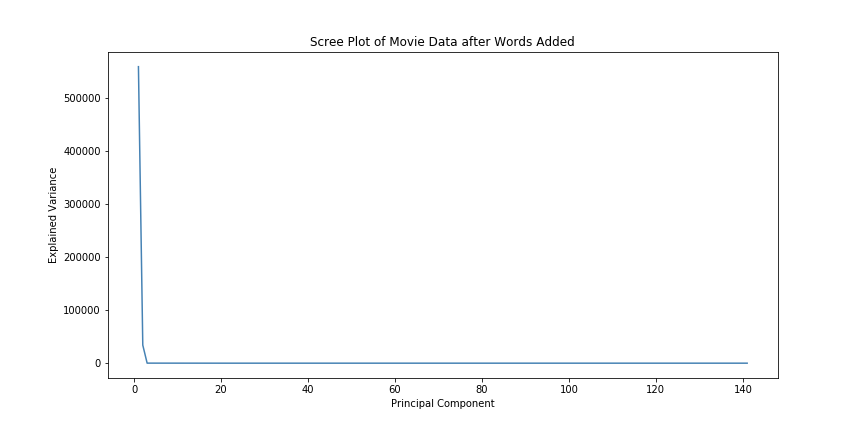
\includegraphics[width=\textwidth]{scree_whole}
\caption{\label{fig:scree_whole}Scree plot of principal components.}
\end{figure}

\begin{figure}%[H]
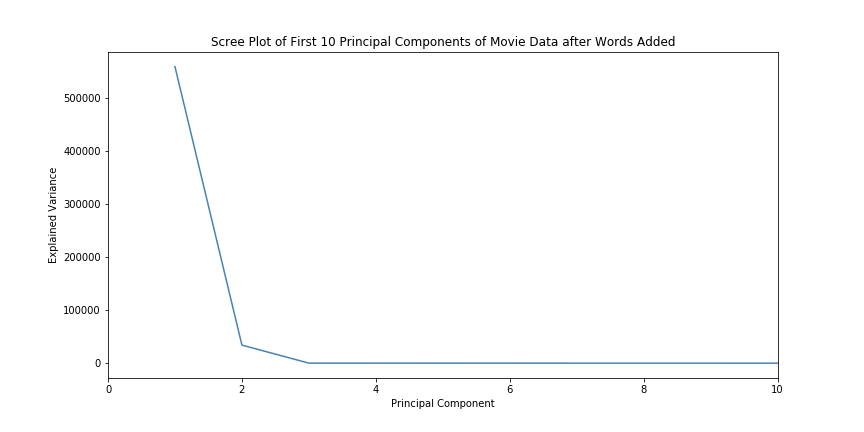
\includegraphics[width=\textwidth]{scree_first_10}
\caption{\label{fig:scree_first_10}Scree plot of first 10 principal components.}
\end{figure}

As Figure \ref{fig:pca_var_explained} shows, the first two princpal components account for almost 100\% of the variance in the dataset. The rotated data points are plotted along Princpal Components 1 and 2 in Figure \ref{fig:pc1_pc2}.

\begin{figure}%[H]
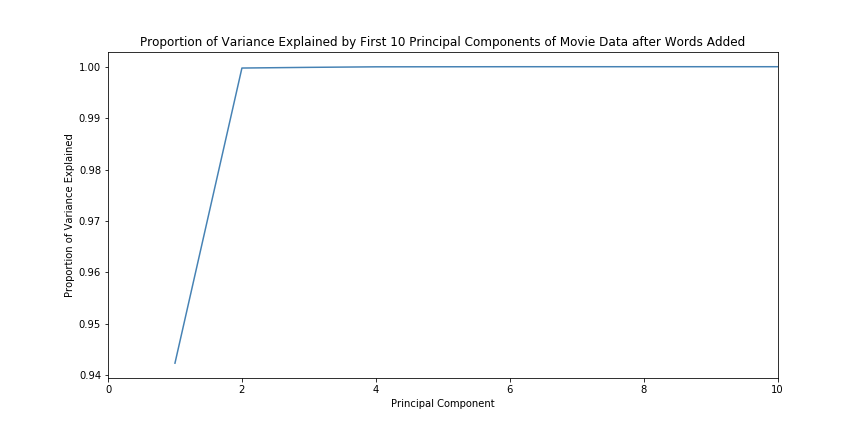
\includegraphics[width=\textwidth]{pca_var_explained}
\caption{\label{fig:pca_var_explained}Cumulative proportion of variance explained by first 10 principal components.}
\end{figure}

\begin{figure}%[H]
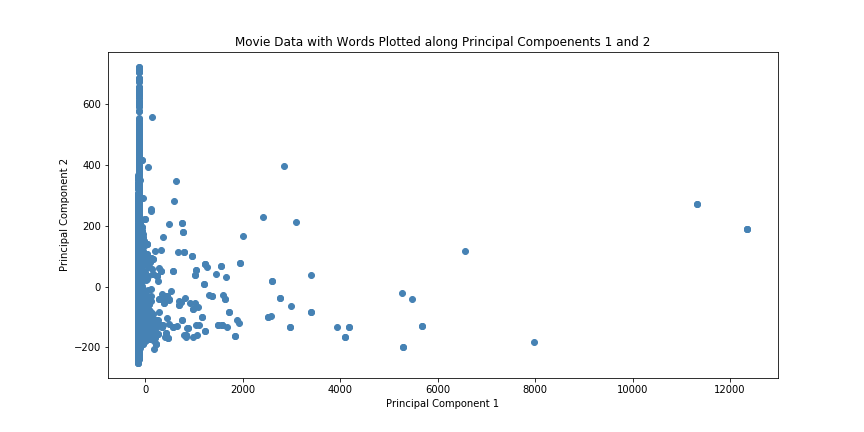
\includegraphics[width=\textwidth]{pc1_pc2}
\caption{\label{fig:pc1_pc2}Rotated data plotted along Princpal Components 1 and 2.}
\end{figure}

\subsection{Classification without Posters}
\label{section:class_no_posters_results}

After the first round of hyperparameter search, the ridge classifier performed best with $\alpha=0$, the support vector classifier with $C=100$, and the kNN classifier with 1 neighbor. The decision tree classifier had no hyperparameters of interest. The results of feature selection and tuning on the training data are provided in Table \ref{table:class_no_poster_results}. Table \ref{table:class_no_poster_test_results} details the testing MAE and RMSE for each tuned model and feature selection scheme from Table \ref{table:class_no_poster_results}. As an example, Table \ref{table:class_no_poster_results} shows that a kNN classififier with 1 neighbor and ANOVA F-value feature selection had a validation error of 0.32484, and Table \ref{table:class_no_poster_test_results} shows that that same model had a testing MAE of 1.18699 and RMSE of 2.20421. The hyperparameters used in these models are:

\begin{itemize}
\item ridge: $\alpha=0$
\item SVC: $C=100$
\item kNN: 1 neighbor
\end{itemize}

The results show that a support vector classifier with $C=100$ and feature selection using mutual information is the best classifier, with an MAE of 0.87154 and an RMSE of 1.72500. The predictions of this classifier are depicted in Figure \ref{fig:no_poster_test_results}. This feature selection scheme chose 10 features: \texttt{popularity}, \texttt{vote\_count}, \texttt{Horror}, \texttt{Music}, \texttt{Thriller}, \texttt{overview\_len}, \texttt{day}, \texttt{take}, \texttt{direct}, and \texttt{evil}. The last three features correspond to the presence of words as described in \S \ref{section:words_results}.

\begin{table}
\resizebox{\textwidth}{!}{%
\begin{tabular}{l|ll|ll|l|ll}
\textbf{Classifier $\rightarrow$} & \textbf{Ridge} & \textbf{} & \textbf{SVC} & \textbf{} & \textbf{Decision Tree} & \textbf{kNN} & \textbf{} \\
\textbf{Feature Selection Scheme $\downarrow$} & \textbf{$\alpha$} & \textbf{MAE} & \textbf{$C$} & \textbf{MAE} & \textbf{MAE} & \textbf{neighbors} & \textbf{MAE} \\ \hline
\textbf{No Selection} & 0 & 1.19740 & 100 & 0 & 0 & 1 & 0 \\
\textbf{Chi-Squared Statistics} & 0.1 & 1.40022 & 10 & 0 & 0 & 1 & 0 \\
\textbf{ANOVA F-value} & 0 & 1.40130 & 100 & 1.15998 & 0.27983 & 1 & 0.32484 \\
\textbf{Mutual Information} & 0 & 1.41811 & 10 & 0 & 0 & 1 & 0
\end{tabular}%
}
\caption{\label{table:class_no_poster_results}Results of feature selection and hyperparameter tuning without posters.}
\end{table}

\begin{table}
\resizebox{\textwidth}{!}{%
\begin{tabular}{l|ll|ll|ll|ll}
\textbf{Classifier $\rightarrow$} & \textbf{Ridge} & \textbf{} & \textbf{SVC} & \textbf{} & \textbf{Decision Tree} & \textbf{} & \textbf{kNN} & \textbf{} \\
\textbf{Feature Selection Scheme $\downarrow$} & \textbf{MAE} & \textbf{RMSE} & \textbf{MAE} & \textbf{RMSE} & \textbf{MAE} & \textbf{RMSE} & \textbf{MAE} & \textbf{RMSE} \\ \hline
\textbf{No Selection} & 1.46016 & 2.14438 & 0.95772 & 1.80289 & 0.95610 & 1.94309 & 1.07805 & 1.94518 \\
\textbf{Chi-Squared Statistics} & 1.36260 & 1.98449 & 0.90569 & 1.76460 & 1.01789 & 2.01377 & 1.07967 & 1.96638 \\
\textbf{ANOVA F-value} & 1.38537 & 2.03386 & 1.43577 & 2.15836 & 1.14472 & 2.15271 & 1.18699 & 2.20421 \\
\textbf{Mutual Information} & 1.46992 & 2.04661 & 0.87154 & 1.72500 & 1.03089 & 1.96886 & 1.08618 & 1.96804
\end{tabular}%
}
\caption{\label{table:class_no_poster_test_results}Classifier testing errors on classification without posters.}
\end{table}

\begin{figure}%[H]
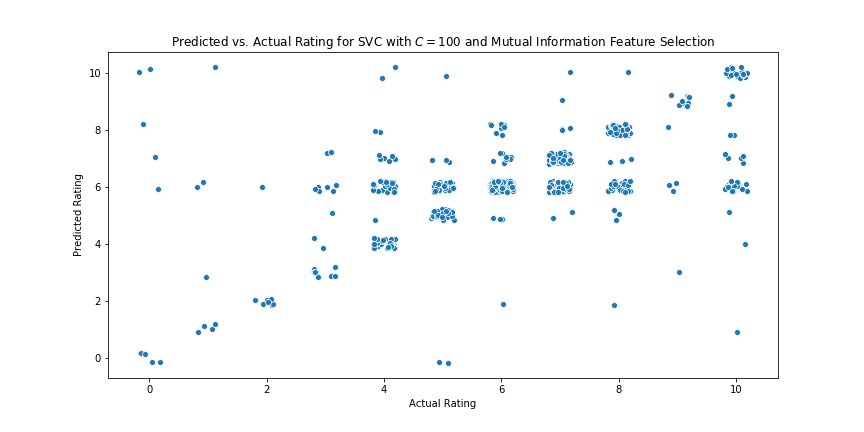
\includegraphics[width=\textwidth]{no_poster_test_results}
\caption{\label{fig:no_poster_test_results}Results of classification without posters with $U(-0.2, 0.2)$ jittering on both axes.}
\end{figure}

\subsection{Classifying Movie Posters}

This section created multiple neural networks, both convolutional and otherwise. The non-convolutional neural networks were trained on the flattened image arrays and contained different numbers dense hidden layers. Both softmax and sigmoid activation functions for the final layer were considered. The convolutional NNs were trained on the 3-dimensional image arrays, which were then flattened and run through non-convolutional dense layers. All NNs in this section use the Adam optimizer and categorical cross-entropy loss.

Some neural network models analyzed in this section predicted all fours or all zeros, including one of the convolutional NNs. Figure \ref{fig:cnn_all_fours_first_layer} shows the features picked out by the first convolutional layer of this network when predicting on the poster in Figure \ref{fig:isle_of_dogs_poster}.

\begin{figure}%[H]
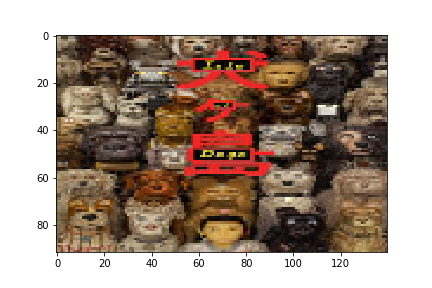
\includegraphics[width=\textwidth]{isle_of_dogs_poster}
\caption{\label{fig:isle_of_dogs_poster}Original poster for picturing CNN layer features.}
\end{figure}

\begin{figure}%[H]
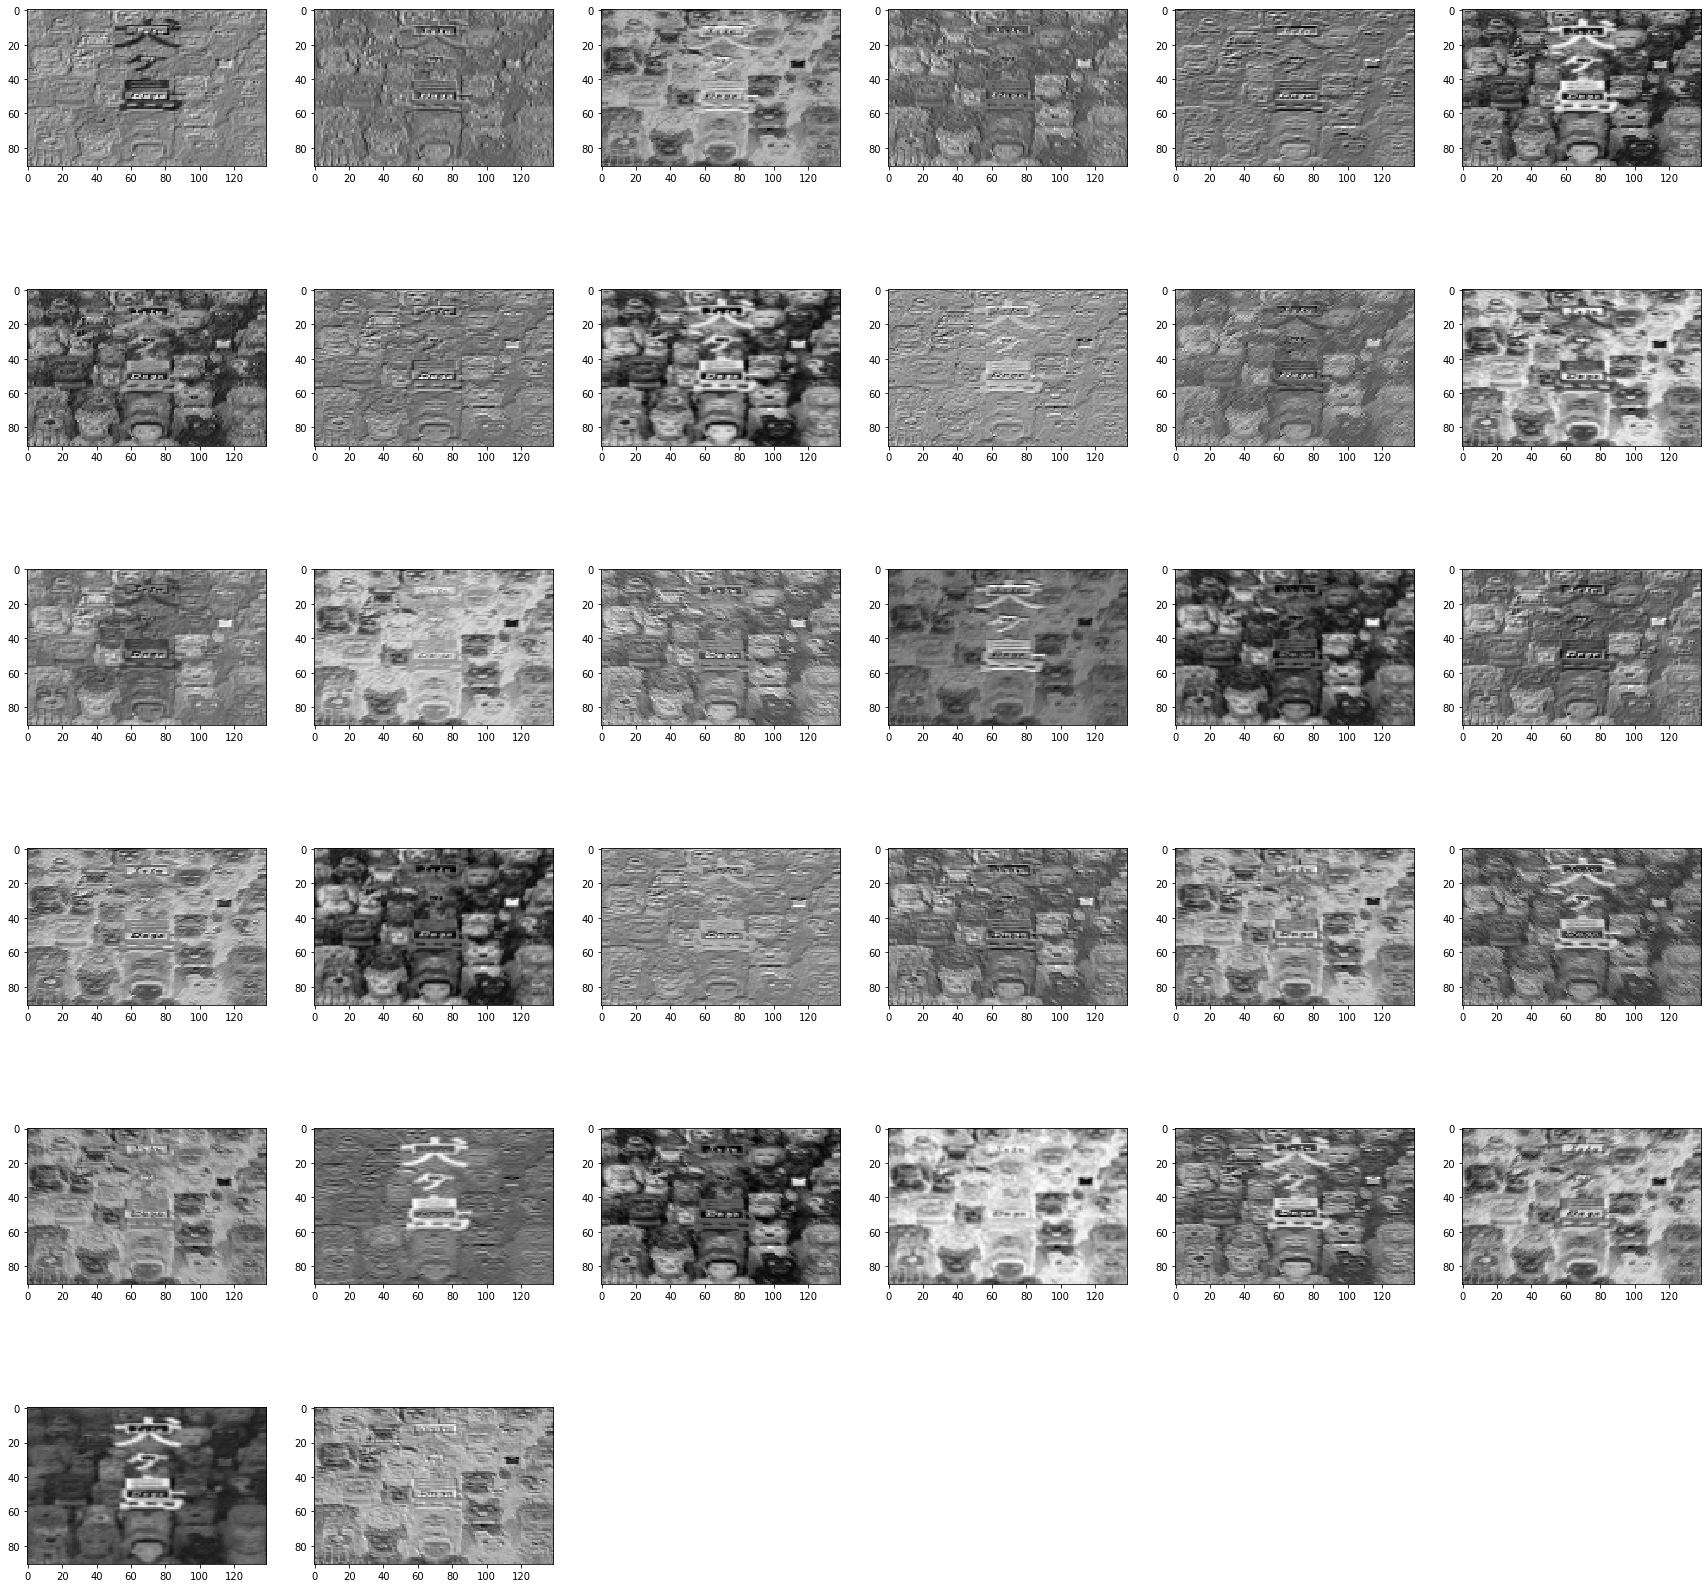
\includegraphics[width=\textwidth]{cnn_all_fours_first_layer}
\caption{\label{fig:cnn_all_fours_first_layer}All-fours CNN first layer features.}
\end{figure}

A better CNN trained in this section, summarized in Figure \ref{fig:better_cnn_summary}, predictions with an MAE of 1.96941 and an RMSE of 2.62073. The features learned by the input layer of this model are shown in Figure \ref{fig:better_cnn_first_layer}.

\begin{figure}%[H]
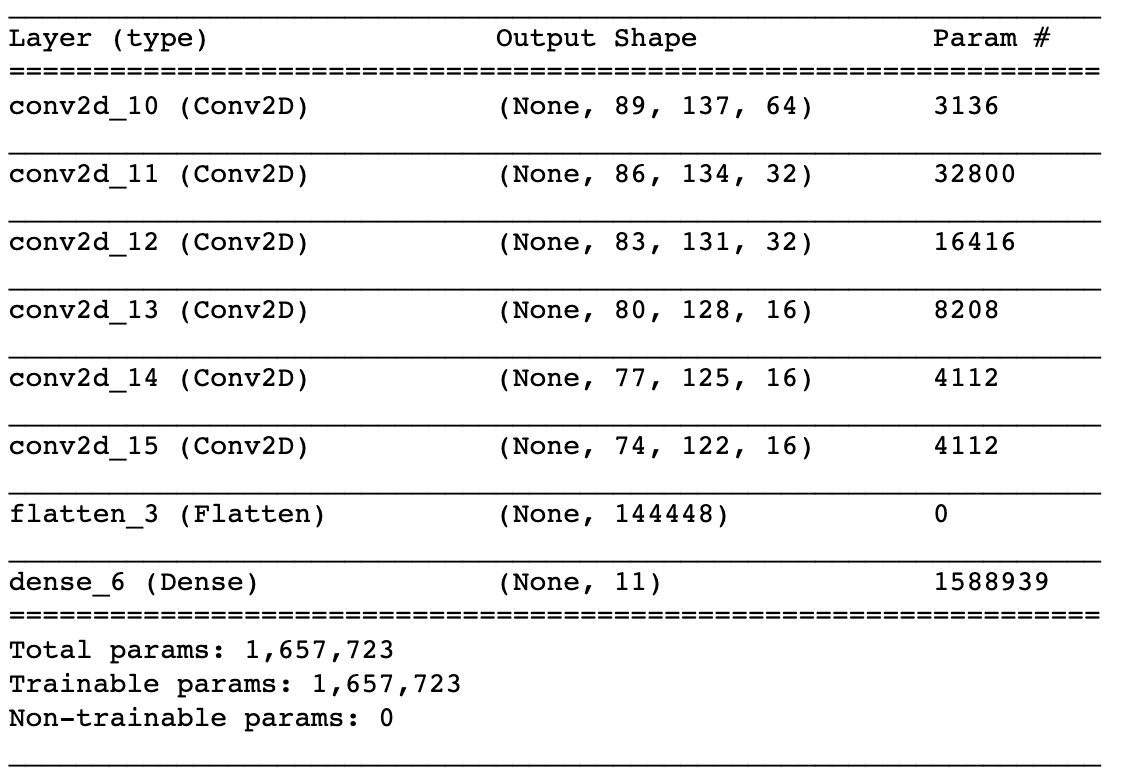
\includegraphics[width=\textwidth]{better_cnn_summary}
\caption{\label{fig:better_cnn_summary}Better CNN model summary.}
\end{figure}

\begin{figure}%[H]
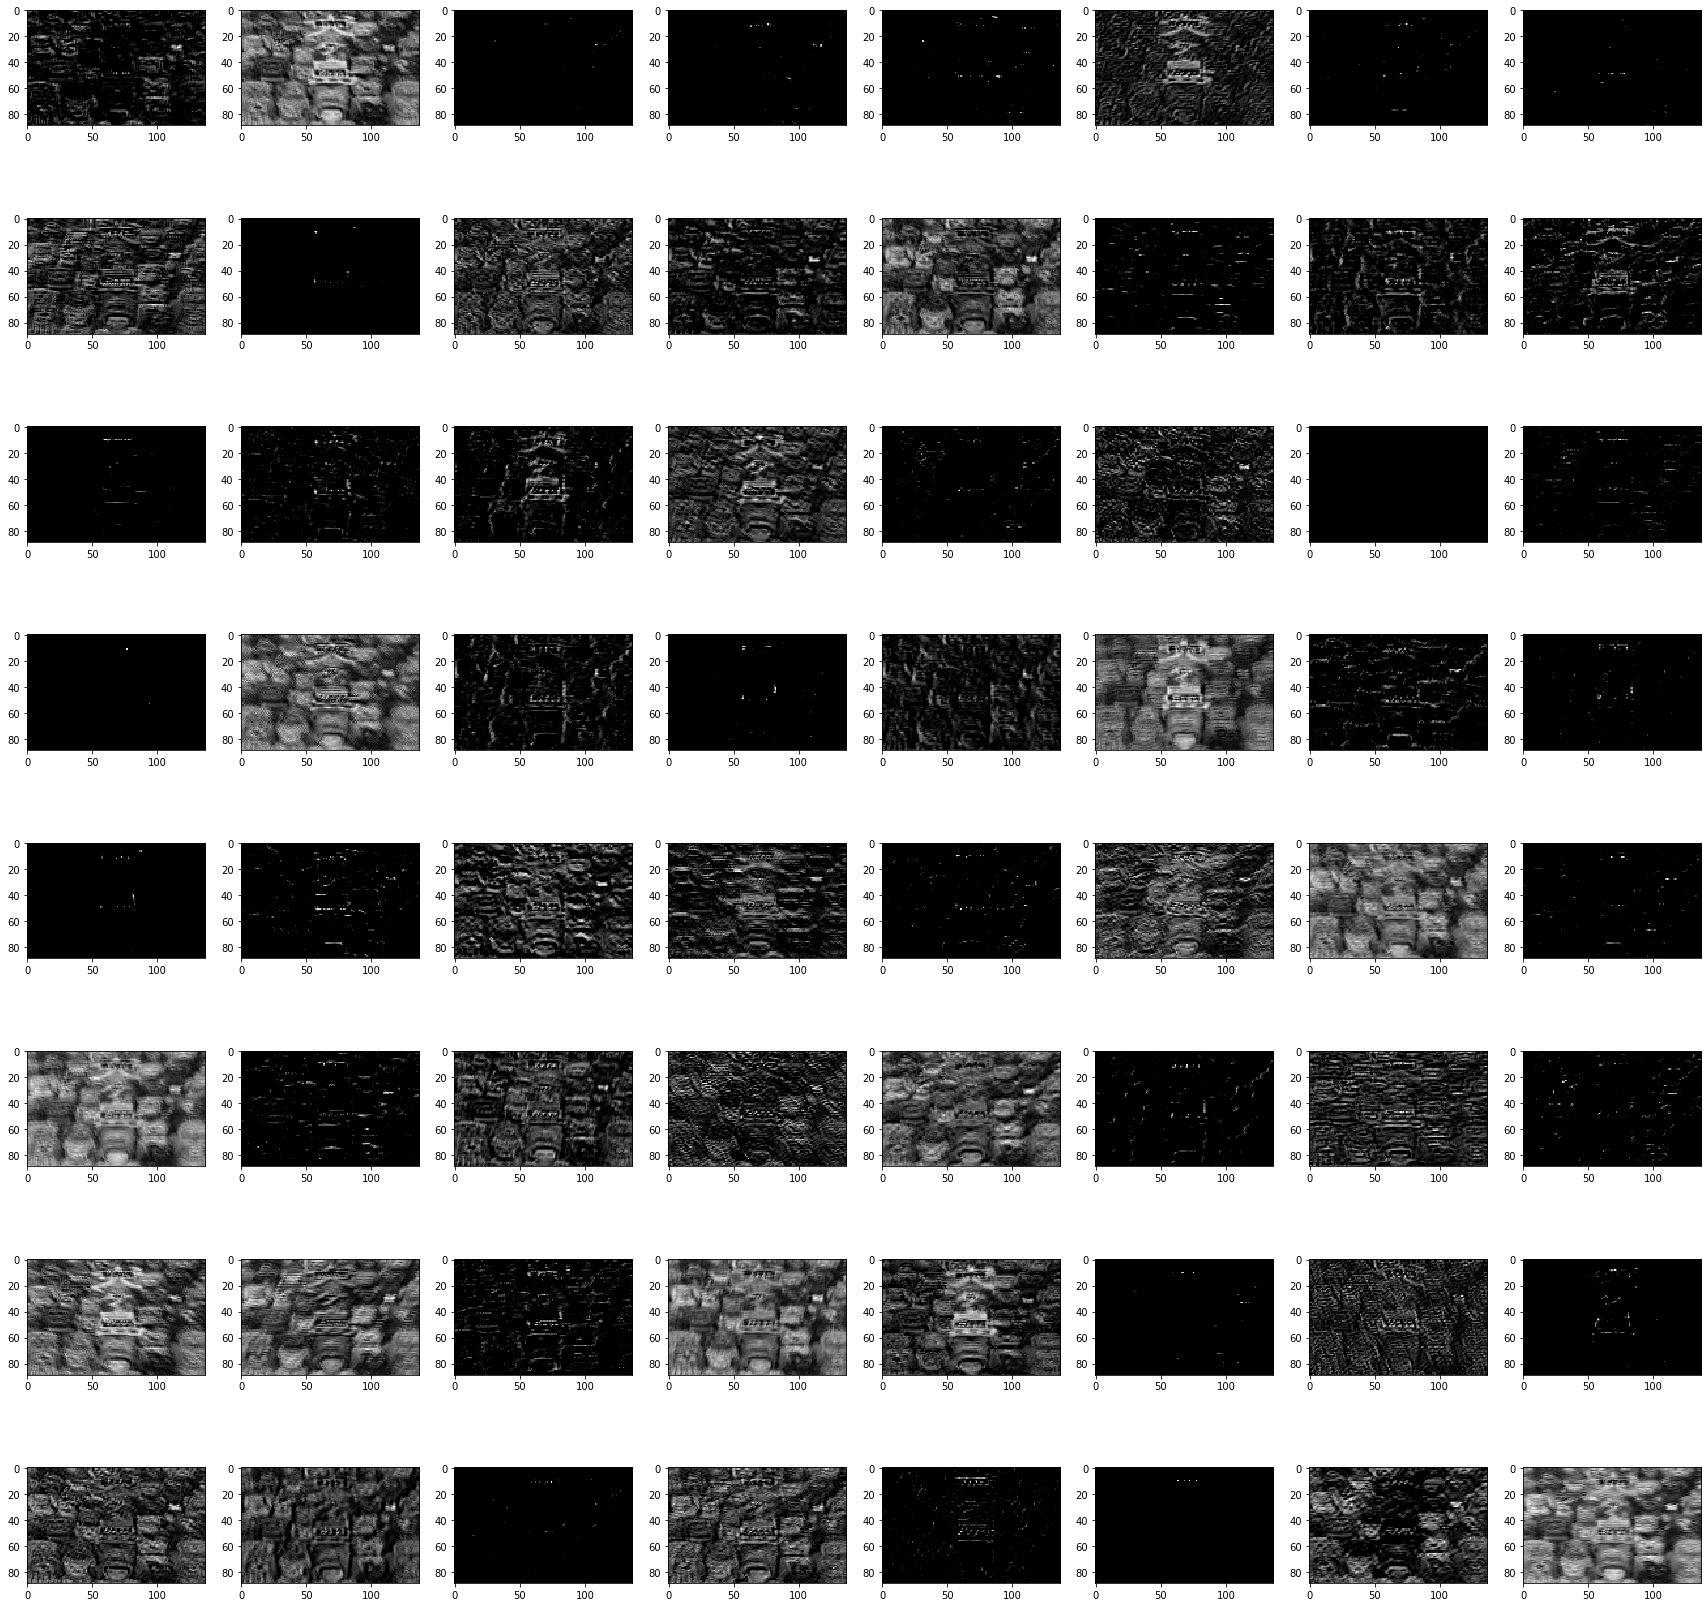
\includegraphics[width=\textwidth]{better_cnn_first_layer}
\caption{\label{fig:better_cnn_first_layer}Better CNN input layer features.}
\end{figure}

What is interesting to note is that the all-fours CNN learns a more diffuse representation and a wider variety of features in the model. Figure \ref{fig:cnn_all_fours_first_layer} highlights grays of different hues and some of the neurons highlight textual features in the image. Contrast this to Figure \ref{fig:better_cnn_first_layer}, which shows several edge detectors (the mostly-black frames) and only a few neurons that learn more textual features. None of the neurons in the better CNN appear to recognize different shades of gray. This indicates that perhaps edge detection is a better method of learning features for predicting movies. Lower layers of this CNN learned to detect different textures in addition to edges, as shown in the Figure \ref{fig:better_cnn_fifth_layer}.

\begin{figure}%[H]
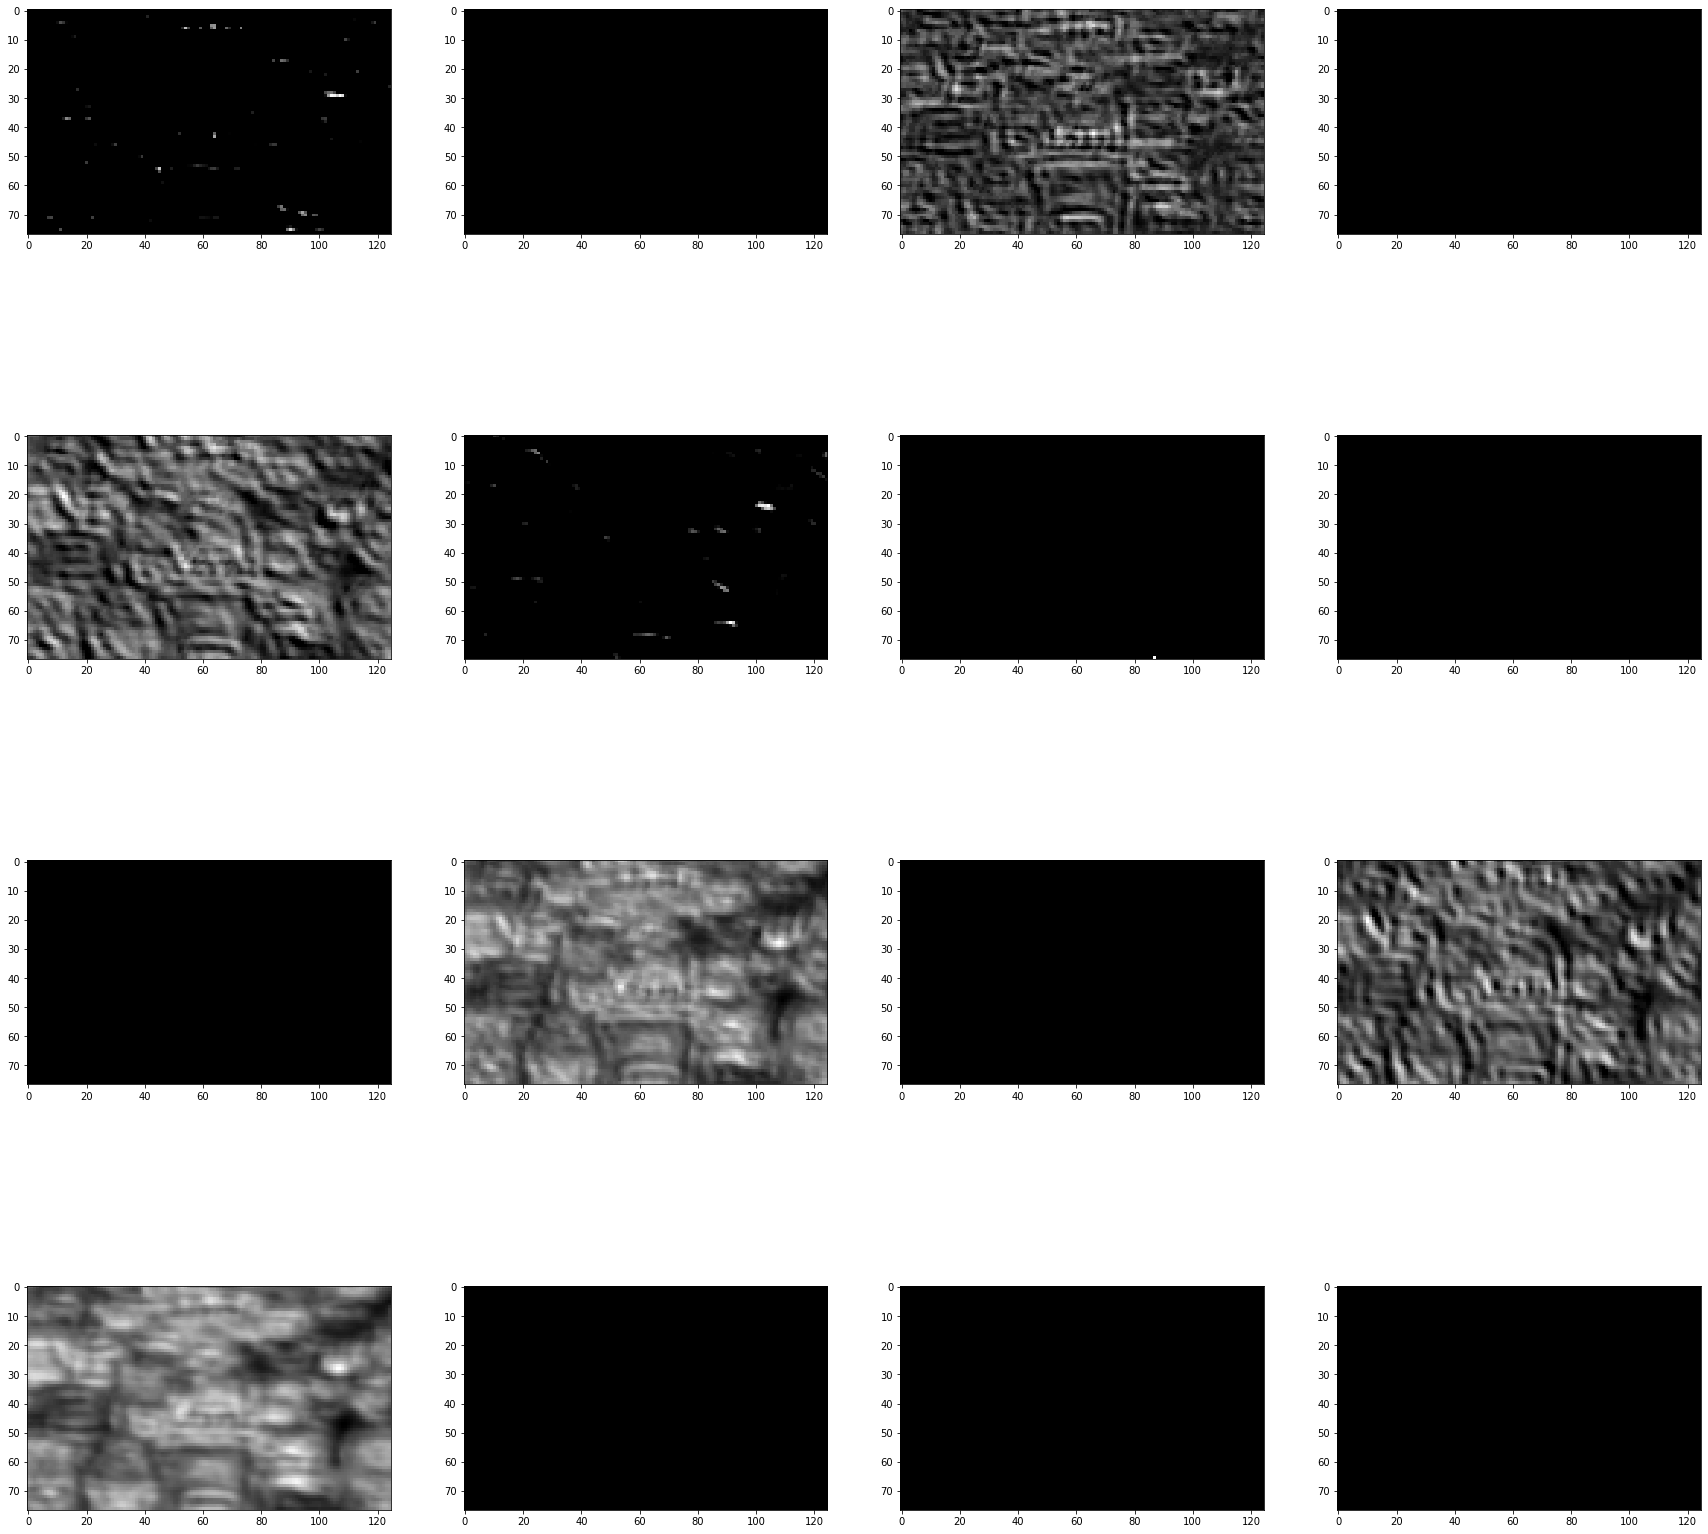
\includegraphics[width=\textwidth]{better_cnn_fifth_layer}
\caption{\label{fig:better_cnn_fifth_layer}Better CNN fifth layer features.}
\end{figure}

Several non-convolution neural networks were tested, including 11 non-convolutional fully-connected networks (FCNNs) with 1 hidden layer trained over 100 epochs with batch size 16. The MAEs for these networks for different numbers of hidden units are provided in Table \ref{table:fcnn_maes}.

\begin{table}
\begin{center}\begin{tabular}{c|l}
\textbf{Number of Hidden Units} & \textbf{MAE} \\ \hline
1 & 1.989720549637178 \\
2 & 1.9078307858576502 \\
4 & 1.6101929905820598 \\
8 & 2.181723019916628 \\
16 & 1.712555195306469 \\
32 & 1.5834213370387524 \\
64 & 1.492082754361587 \\
128 & 1.492082754361587 \\
256 & 2.388825073336421 \\
512 & 2.0121877412382276 \\
1024 & 1.9250671607225567 \\
\end{tabular}\end{center}
\caption{\label{table:fcnn_maes}MAEs for different numbers of hidden units in non-convolutional FCNNs with 1 hidden layer.}
\end{table} 

\section{Conclusions}

Several interesting conclusions can be drawn from the analysis of this project, with two salient points:
\begin{enumerate}
\item fully-connected neural networks trained on flattened images appear to be better predictors than do convolutional neural networks, and
\item movie posters are not the best predictors of ratings
\end{enumerate}

To the first, compare the errors noted in Table \ref{table:fcnn_maes} to those noted for the CNNs. The difference is clearly in favor of the FCNNs on this score. One possible reason for this, however, may be the lack of depth of the CNNs trained in this analysis. Traditionally, deep learning performed with CNNs is done with networks of 15+ layers, a level clearly not broached in this analysis due to computation power limitations. So while, at a shallow level, it appears that the FCNNs have the upper hand, the convolutional networks may be able to outperform them at the level of deep learning.

To the second, we observed that when comparing even the best networks trained in this analysis that they do not outperform the classifiers trained on other pieces of movie data from the \texttt{movies} dataframe. This is perhaps a reasonable conclusion as posters are more determinant of a person's desire to see a movie in the first place, and so likely have a lesser effect on their \textit{rating} of that movie after having seen it. 

The principal components analysis reveals that while the data are largely well-represented by two principal components, which together explain almost 100\% of the variance in the data, there is quite a lot of variance among the sample points themselves. This is observed in the scale of the axes of Figures \ref{fig:scree_whole} and \ref{fig:pc1_pc2}. Figure \ref{fig:pc1_pc2} shows in particular that there is a more uniform density of points along different values of Principal Component 2 compared to a more right-skewed distribution along Principal Component 1.

Some suggestions for further analysis include training deeper networks on the 3-tensor posters in order to see if these can outperform the FCNNs trained herein, and using posters perhaps as a predictor of box office-success. As noted above, posters are usually more involved in a person's decision to see a movie, and so the profits of a movie are likely better predicted by posters than are the ratings.

% \begin{appendices}
\newpage

\addcontentsline{toc}{section}{References}
\bibliographystyle{unsrt} % We choose the "plain" reference style
\bibliography{references.bib}

\newpage

\appendix
\section{Appendix: Word Signficiance Table}
\label{appendix:word_signif_table}

\begin{table}[H]
\begin{tabular}[t]{l|l}
\textbf{Word}        & \textbf{p-value} \\ \hline
this        & 0.001    \\
after       & 0.006    \\
known       & 0.003    \\
% side        & 0.0      \\
killer      & 0.001    \\
business    & 0.019    \\
seem        & 0.009    \\
follows     & 0.028    \\
become      & 0.03     \\
house       & 0.003    \\
% meets       & 0.0      \\
aunt        & 0.017    \\
each        & 0.012    \\
making      & 0.001    \\
place       & 0.002    \\
% only        & 0.0      \\
foot        & 0.009    \\
% perform     & 0.0      \\
lore        & 0.036    \\
give        & 0.038    \\
found       & 0.031    \\
front       & 0.047    \\
women       & 0.024    \\
ours        & 0.035    \\
behind      & 0.001    \\
kill        & 0.004    \\
attempt     & 0.01     \\
disco       & 0.003    \\
mysterious  & 0.004    \\
king        & 0.015    \\
less        & 0.013    \\
turn        & 0.049    \\
begin       & 0.001    \\
years       & 0.002    \\
range       & 0.001    \\
discover    & 0.011    \\
\end{tabular}
\begin{tabular}[t]{l|l}
\textbf{Word}        & \textbf{p-value} \\ \hline
through     & 0.005    \\
take        & 0.012    \\
% group       & 0.0      \\
film        & 0.004    \\
gain        & 0.041    \\
% great       & 0.0      \\
trip        & 0.02     \\
care        & 0.009    \\
couple      & 0.049    \\
even        & 0.042    \\
party       & 0.027    \\
cove        & 0.003    \\
down        & 0.004    \\
% dire        & 0.0      \\
story       & 0.01     \\
father      & 0.04     \\
disc        & 0.009    \\
under       & 0.047    \\
ller        & 0.003    \\
busi        & 0.008    \\
direct      & 0.007    \\
light       & 0.002    \\
does        & 0.018    \\
dangerous   & 0.002    \\
break       & 0.007    \\
evil        & 0.005    \\
host        & 0.002    \\
survive     & 0.001    \\
meet        & 0.037    \\
realize     & 0.03     \\
% murder      & 0.0      \\
college     & 0.014    \\
documentary & 0.005    \\
self        & 0.02     \\
super       & 0.042    \\
across      & 0.006    \\
\end{tabular}
\begin{tabular}[t]{l|l}
\textbf{Word}        & \textbf{p-value} \\ \hline
rough       & 0.004    \\
cross       & 0.002    \\
hard        & 0.001    \\
brother     & 0.037    \\
childhood   & 0.001    \\
small       & 0.018    \\
director    & 0.02     \\
% feat        & 0.0      \\
danger      & 0.005    \\
dang        & 0.002    \\
between     & 0.003    \\
mean        & 0.003    \\
christmas   & 0.016    \\
year        & 0.018    \\
press       & 0.046    \\
ross        & 0.005    \\
dark        & 0.001    \\
% follow      & 0.0      \\
document    & 0.002    \\
% first       & 0.0      \\
brea        & 0.009    \\
anger       & 0.001    \\
strange     & 0.005    \\
hunt        & 0.002    \\
% secret      & 0.0      \\
takes       & 0.004    \\
fall        & 0.014    \\
% music       & 0.0      \\
which       & 0.029    \\
soon        & 0.002    \\
know        & 0.017    \\
% them        & 0.0      \\
wing        & 0.032    \\
% comedy      & 0.0      \\
form        & 0.001    \\
test        & 0.02     \\
cover       & 0.026    \\
mall        & 0.04     \\
\end{tabular}
\caption{\label{table:word_p_values}Words with statistically significant presences and corresponding p-values.}
\end{table}

% \end{appendices}

\end{document}